% Figure 6 dense LaTeX assembly snippet.
% Generate the panel PDFs first:
%   Rscript scripts/build_figure6_consequence_density.R
%
% This snippet is intentionally kept outside main.tex until the R-rendered
% assets exist, so the current manuscript remains compilable.

\begin{figure*}[t]
  \centering
  \begin{minipage}[t]{0.49\linewidth}
    \textbf{a}\par\vspace{1pt}
    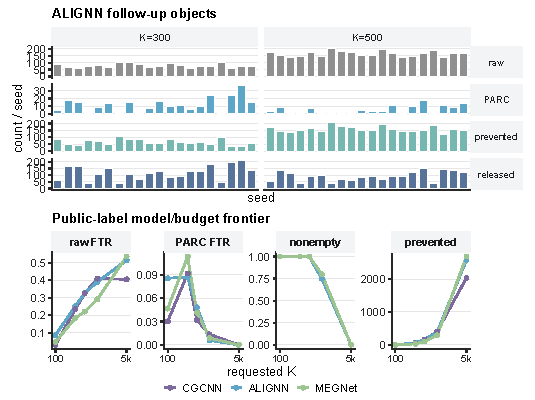
\includegraphics[width=\linewidth]{figure6_assets/rebuild/figure_6a_materials_artifact_grid.pdf}
  \end{minipage}\hfill
  \begin{minipage}[t]{0.49\linewidth}
    \textbf{b}\par\vspace{1pt}
    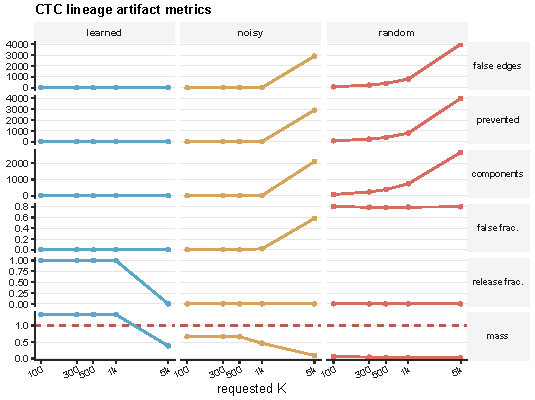
\includegraphics[width=\linewidth]{figure6_assets/rebuild/figure_6b_ctc_artifact_grid.pdf}
  \end{minipage}

  \vspace{2pt}
  \begin{minipage}[t]{0.49\linewidth}
    \textbf{c}\par\vspace{1pt}
    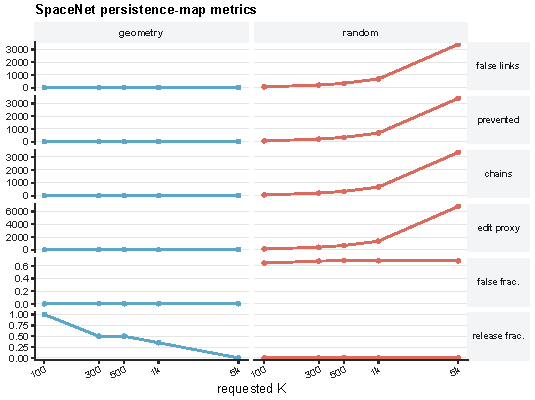
\includegraphics[width=\linewidth]{figure6_assets/rebuild/figure_6c_map_audit_grid.pdf}
  \end{minipage}\hfill
  \begin{minipage}[t]{0.49\linewidth}
    \textbf{d}\par\vspace{1pt}
    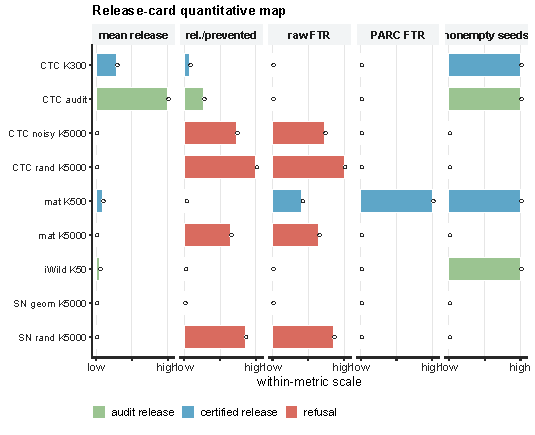
\includegraphics[width=\linewidth]{figure6_assets/rebuild/figure_6d_release_card_quant_grid.pdf}
  \end{minipage}
  \caption{\textbf{Release decisions change downstream scientific artifacts without new human labels.} a, Retrospective public-label materials follow-up emulation combines seed-level raw/PARC/prevented queue distributions with public-label model/budget frontiers. b, CTC official-ground-truth lineage consequences are shown as source-resolved \(K\)-sweeps of false-edge, component, release and evidence-mass metrics. c, SpaceNet 7 building-persistence consequences are shown as source-resolved \(K\)-sweeps of false-link, map-edit and release metrics. d, Release-card summaries are encoded as quantitative metric grids rather than claim-status tiles.}
  \label{fig:nohumanconsequence}
\end{figure*}
